\section{Experimental Results}
\label{sec:experiments}

\subsection{Evaluation Measure}

Because we aim to take into account the findings of Parnin and Orso
\cite{AutoHelp}, our evaluation of fault localizations is based on a
\emph{pessimistic absolute rank} of the highest ranked faulty
statement.  That is, for each set of suspiciousness metrics computed,
our measure of effectiveness is the \emph{worst possible position} at
which the first faulty statement can be reached, when examining the
code in suspiciousness-ranked order.\footnote{As usual since at least
the work of Reneiris and Reiss\cite{NearNeighbor}, we consider
reaching \emph{any} faulty statement to be sufficient.}  For example,
if ten statements all receive a suspiciousness score of 1.0 (the
highest possible suspiciousness), and one of these is the fault, we
assign this localization a rank of 10; an unlucky programmer might
examine this statement last of the ten highest-ranked statements.
Pessimistic rank nicely distinguishes this result from another
localization that also places the bug at score 1.0, but gives twenty
statements a 1.0 score. In our view, following Parnin and Orso
\cite{AutoHelp}, the most important goal of a localization is to
direct the developer to a faulty statement as rapidly as possible,
ignoring the size of the entire program or even of the faulty
execution.  

\subsection{SIR Programs}

\begin{figure*}
  \centering
  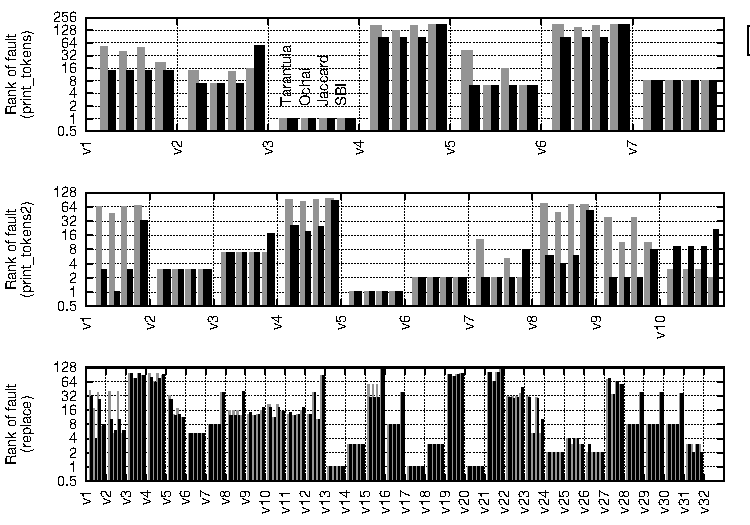
\includegraphics[width=1.8\columnwidth]{siemens1}
  \caption{First Set of SIR Results}
  \label{fig:allSIR1}
\end{figure*}

\begin{figure*}
  \centering
  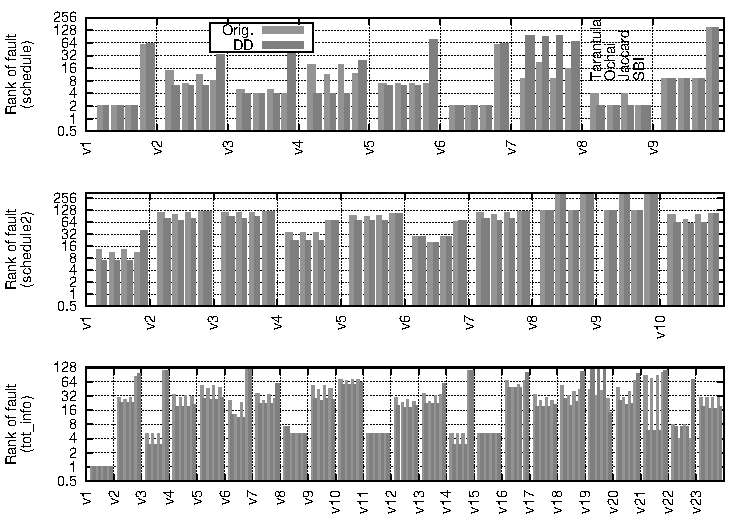
\includegraphics[width=1.8\columnwidth]{siemens2}
  \caption{Second Set of SIR Results}
  \label{fig:allSIR2}
\end{figure*}


\begin{table*}
\begin{center}
\begin{tabular}{|c||c|c|c|c|c||c|c|c|c|c|}
\hline
\hline
& \multicolumn{5}{|c|}{With AMPLE} & \multicolumn{5}{|c|}{Without AMPLE} \\
\hline
Subject & Avg. & Avg. (DD) & \#Better & \#Same & \#Worse & Avg. & Avg. (DD) & \#Better & \#Same & \#Worse \\
\hline
\hline
{\tt print\_tokens} & 59.7 & 36.4 & 19 & 15 & 1 & 59.7 & 29.7 & 18 & 10 & 0 \\
\hline
{\tt print\_tokens2} & 26.8 & 9.2 & 23 & 20 & 7 & 27.0 & 5.8 & 19 & 17 & 4 \\
\hline
{\tt replace} & 26.5 & 24.6 & 38 & 98 & 19 & 24.5 & 21.8 & 37 & 76 & 11 \\
\hline
{\tt schedule} & 13.1 & 22.7 & 18 & 16 & 11 & 7.7 & 14.3 & 18 & 14 & 4 \\
\hline
{\tt schedule2} & 100.3 & 88.4 & 29 & 17 & 4 & 92.4 & 76.6 & 28 & 12 & 0 \\ 
\hline
{\tt tot\_info} & 34.1 & 26.05 & 82 & 24 & 9 & 29.7 & 17.7 & 75 & 16 & 1\\
\hline
\hline
{\bf Total} & & & 209 & 190 & 51 & & & 195 & 145 & 20 \\
\hline
\hline
\end{tabular}
\end{center}
\caption{SIR Fault Rank Change Result Frequencies}
\label{tab:avgimproved}
\end{table*}

Our initial experiments use the Siemens/SIR \cite{doESE05,Siemens}
suite programs studied in many previous papers on fault localization,
in particular the classic evaluation of the Tarantula technique
\cite{Tarantula}.  These subjects provide a large number of faults,
reasonable-sized test suites, and have historically been used to
evaluate localization methods.

Of the seven Siemens programs considered in the empirical evaluation
of Tarantula, only one was unsuitable for delta debugging: TCAS takes
as input a fixed-size vector of integers, and therefore its inputs
cannot be easily decomposed.  For the remainder of the programs, the
input is easily considered as either 1) a sequence of characters or 2)
a sequence of lines, when character-level delta debugging is not
efficient (and so unlikely to be chosen by users in practice), which
was required for the {\tt tot\_info} subject.  In all cases, reduction
took on average less than three seconds per failing test case, an essentially
negligible computational cost.



We evaluated our proposal by 1) first computing the fault ranking for
each version of each subject by the five formulas then 2) performing
the same computation, but using only reduced (by delta-debugging)
versions of the failing tests.  Reduction was performed using Zeller's
delta-debugging scripts, available on the web, and comparing the output
of the original (correct) version of the program and the faulty
version as a pass/fail oracle.

Figures \ref{fig:allSIR1} and \ref{fig:allSIR2} show the
results\footnote{Version 32 of {\tt replace} is missing because the
fault relies on the library definition of {\tt isalnum}, and is no
longer present on modern Linux systems, as we determined after
communicating with Gregg Rothermel and the SIR maintainers.}.  The
lighter shaded bars show the ranking of the fault, without any
reduction.  The darker bars show the ranking after delta-debugging all
failures.  The graphs are shown in log-scale due to the range of
rankings involved.  In many cases, reducing test cases before
localizing improved the ranking of the fault by a factor of two or
more.  Results for individual subject vary: for {\tt print\_tokens},
the average ranking for faults, over all bugs and all formulas, is
59.5 without reduction, and 36.4 with reduction.  The result is
improved by reduction in 19 cases, remains the same in 15 cases, and
is worse in 1 case.  These numbers improve to 29.8 average ranking, 18
improvements, and 10 unchanged results if we ignore AMPLE scores.
Table \ref{tab:avgimproved} shows similar data for all the SIR
subjects.  

For all but one subject, average scores were better after reduction.
That one subject, {\tt schedule} has worse results due to faulty
version 7.  This version, unlike all other SIR bugs, is not actually a
single fault.  Instead, two independent (but identical in text)
changes to the code exist, and reduction takes many test cases that
execute both faulty lines, and removes one of them.  This results in
both faulty lines getting worse ranks.  In other words, our first
assumption was violated.  However, this is a somewhat unusual
``multiple fault'' case in that the two faults are identical incorrect
statements, and in some sense interchangeable --- in a more typical
multi-fault setting, we expect that faults will tend to be independent
and a test case for one fault will often not cover the other fault in
the first place.  That is, our belief is that the typical multi-fault
setting has multiple faults, but test cases that involve only one
fault.  In this example, however, one fault executed in 19 of the 27
failing test cases, the other executed in 24, and \emph{both} executed
in 16: after reduction, of course, since either fault will cause a
problem, both were covered less frequently, and no test executed both.
The other non-AMPLE cases where the ranking was worse seem to all be
due to decreasing input size leading to some increase in code
coverage, due to the structure of the software.  One simple solution
for this problem would be to modify the delta-debugging scripts to
reject reductions that cover code not covered by the original failing
test case.  Even without such a modification, if we ignore AMPLE
results, improvement in fault rank was 1.3 times as common as no change
in rank, and \emph{nearly 10 times as common as worse rank for the
fault.}  In addition to the frequency of improvement of fault rank, it
is also important to examine the degree of improvement (or the
opposite) provided by reduction.  Table \ref{tab:rankchange} shows,
ignoring AMPLE, the min, max, and average for changes in rank.  With
the exception of the unusual multi-fault program, {\tt schedule} v7,
(which accounts for all worse ranks for {\tt schedule}), the effect
size when reduction improved rank was usually much larger than the
effect size when it gave worse results.  For {\tt replace}, the
subject with the most instances where reduction made fault ranking
worse, we see that the effect size when reduction was harmful was much
smaller than when reduction was helpful.  Furthermore, when reduction
helped, it often improved the ranking of the fault by more than
\emph{optimally} switching formula (the exceptions usually rising from
a poor performance by AMPLE).  That is, we can ask: if we compare
taking the \emph{worst} formula and applying reduction to improve the
localization, how often is this better than switching to the
\emph{best} localization formula for that subject and fault?
Obviously applying reduction is more practical, since we don't know in
advance which formula will perform best, until we know the correct
result.  By this comparison, if we ignore AMPLE, it was better to
apply reduction than switch from \emph{worst} to \emph{best} formula
in 36 cases over all SIR subjects.  It was better to switch formula in
only 22 cases (in the remaining 32 cases these two methods were tied).



\begin{table}
\begin{center}
\begin{tabular}{|c||c|c|c||c|c|c|}
\hline
\hline
& \multicolumn{3}{|c|}{Better} & \multicolumn{3}{|c|}{Worse} \\
Subject & Min & Max & Avg. & Min & Max & Avg \\
\hline
\hline
{\tt print\_tokens} & 6 & 85 & 44.6 & N/A & N/A & N/A \\
\hline
{\tt print\_tokens2} & 3 & 67 & 45.8 & 6 & 6 & 6.0 \\
\hline
{\tt replace} & 1 & 30 & 9.6 & 1 & 3 & 1.4 \\
\hline
{\tt schedule} & 1 & 15 & 4.8 & 85 & 75 & 81.3 \\
\hline
{\tt schedule2} & 4 & 35 & 22.6 & N/A & N/A & N/A \\
\hline
{\tt tot\_info} & 1 & 81 & 14.7 & 3 & 3 & 3.0 \\
\hline
\hline
\end{tabular}
\end{center}
\caption{SIR Fault Rank Change Effect Sizes}
\label{tab:rankchange}
\end{table}

\subsection{SpiderMonkey JavaScript Engine}
SpiderMonkey is the JavaScript Engine for Mozilla, an extremely widely
used, security-critical interpreter/JIT compiler.  SpiderMonkey has
been the target of aggressive random testing for many years now.  A
single fuzzing tool, \texttt{jsfunfuzz} \cite{jsfunfuzz}, is
responsible for identifying more than 1,700 previously unknown bugs in
SpiderMonkey \cite{jsfunfuzzbugs}.  SpiderMonkey is (and was) very
actively developed, with over 6,000 code commits in the period from
1/06 to 9/11 (nearly 4 commits/day).  SpiderMonkey is thus ideal for
evaluating how reduction aids localization when using a sophisticated
random testing system, using the last public release of the
\texttt{jsfunfuzz} tool \cite{jsfunfuzz}, modified for swarm testing \cite{ISSTA12}.
Using a set of faults in SpiderMonkey version 1.6 found with random
testing in previous research \cite{PLDI13}, we show that reduction is
essential for localization of bugs found using random testing, and
that the use of reduction is even somewhat more important than the
choice of localization formula.  


\begin{table}
\begin{center}
\begin{tabular}{|c||c|c|c|c|c||c|c|c|c|c|}
\hline

\hline
Bug\# & Revision Fixed &  \#Failures & {\tt diff} size \\
\hline
\hline
{\tt R60} & 1.16.2.1 & 1 & 115  \\
\hline
{\tt R95} & 1.3.2.3.8 & 7 & 111   \\
\hline
{\tt R115} & 1.4.8.1 & 4 & 592   \\
\hline
{\tt R360} & 3.117.2.6 & 3 & 223  \\
\hline
{\tt R880} & 3.17.2.14 & 28 & 272   \\ 
\hline
{\tt R1172} & 3.208.2.63 & 150 & 214  \\
\hline
{\tt R1294} & 3.241.2.1 & 405 & 80  \\
\hline
{\tt R1543} & 3.36.16.1 & 146 & 169  \\
\hline
{\tt R1561} & 3.37.2.1.4.1.2.2 & 2 & 31  \\
\hline
{\tt R1873} & 3.50.2.29 & 1,041 & 56  \\
\hline
\hline
\end{tabular}
\end{center}
\caption{Spidermonkey Bugs}
\label{tab:spiderbugs}
\end{table}


\begin{figure*}[t]
  \centering
  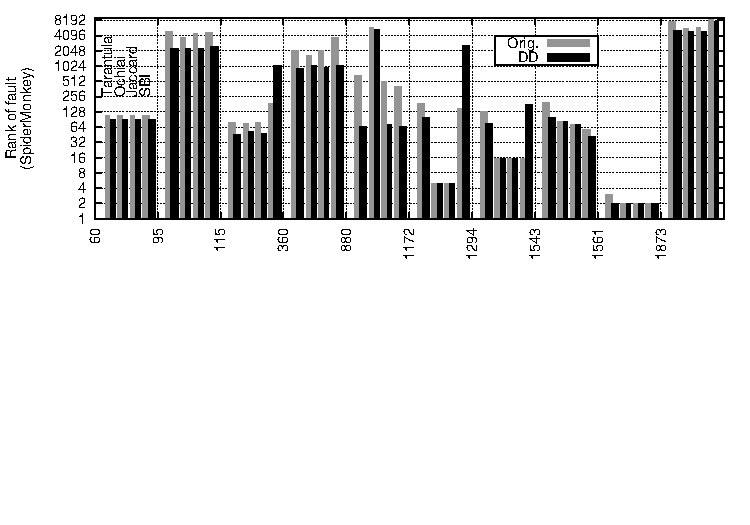
\includegraphics[width=2\columnwidth]{naspidermonkey}
 \vspace{-2.2in}
  \caption{SpiderMonkey Results}
  \label{fig:spidermonkey}

\end{figure*}

Figure \ref{fig:spidermonkey} shows the change in rankings of the
faulty code for 10 SpiderMonkey bugs (Table \ref{tab:spiderbugs}).
These bugs were taken from our PLDI 2013 data set \cite{PLDI13}.  Out
of the 28 bugs studied in that paper we chose 10 random bugs for which, by
hand, we could confirm the true set of faulty lines in the code
commit.  Each bug is identified by the revision number of the commit
in which it was fixed: e.g., R0 maps to revision 1.10.4.1, the first
commit of Spidermonkey changes under consideration. Table
\ref{tab:spiderbugs} shows all bugs studied, the commit version fixing
the bug, the number of failing test cases for that bug (\# Failures),
and the size (in lines) of the fixing commit's {\tt diff}.  The faults
under consideration here are clearly non-trivial (in fact, most fixes
involved changes to multiple source files).  For our localization we
used the original and reduced test cases from PLDI 13 \cite{PLDI13}
plus 720 additional randomly generated \emph{passing} tests generated
using the same tool.

Across these 10 bugs, the average ranking for the first faulty line
encountered was 1,550.7 without reduction, improving to 994.5 with
reduction.  Reduction improved the localization in 33 cases, with a
minimum improvement of 1 ranking and a maximum improvement of 2,137
positions.  The average improvement was 674 positions.  The results
were unchanged in 7 cases. It is important to note that even with such
a challenging setting and real bugs, fault localization with reduction
performs better then fault localization without reduction irrespective
of formula being used: in the \emph{worst} case it performed equally well. It was better to use reduction than to optimally (from worst to
best) switch formula for 5 of the 10 bugs; it was better to switch
formula in 4 cases, and in one case both methods gave the same result.
While the results show that reduction was extremely effective in
improving localization, it is also true that the localization was
\emph{still not very helpful} in many of these cases, considering absolute pessimistic rank as success criteria.  Of course,
SpiderMonkey 1.6 has over 80KLOC, and even reduced failing tests
typically executed over 8,000 lines of code, so a ``poor''
localization may be useful in such a large fault search space.  For 6
of the 10 bugs, all scores after reduction gave a fault ranking $< 128$.



\subsection{Open Source Projects}
\label{sec:opensource}



\begin{table}
{\scriptsize
\begin{center}
\begin{tabular}{|c||c|c|c|c|c||c|c|c|c|c|}
\hline
\hline
& \multicolumn{3}{|c|}{Program Source} & \multicolumn{1}{|c|}{Test Suite} \\
\hline
Subject & \#Classes & \#Methods & SLOC & \#Test cases \\
\hline
\hline
{\tt Apache Commons} & & & & \\
{\tt Validator} & 64 & 578 & 6,033 & 434 \\
\hline
{\tt JExel 1.0.0} & & & & \\
{\tt beta 13} & 43 & 133 & 1,522	 & 344  \\
\hline
{\tt JAxen} & 167 & 1,078 & 12,462 & 2,138\\
\hline
{\tt JParser} & 115 & 178 & 3,046 & 647 \\
\hline
{\tt Apache Commons} & & & & \\
{\tt CLI} & 23 & 208 & 2,667 & 364 \\ 
\hline
\hline
\end{tabular}
\end{center}
}
\caption{Open Source Subject Programs}
\label{tab:opensourcesubs}
\end{table}



Next we applied reduction based localization to five open source Java
programs (shown in Table \ref{tab:opensourcesubs}), generating mutants
for each of the projects to simulate bugs, following previous fault
localization papers \cite{mutant,PureTest}.





 
Our strategy was to create mutants using the approach of Xuan and
Monperrus \cite{PureTest}, using 6 mutant operators.  From each set of
mutants generated, we selected 5 or 6 mutants at random that met the
following criteria: (1) the mutant was killed by at least one test
case and (2) the mutant generated no errors in JUnit test cases.  A
JUnit failure is caused by an unsatisfied assertion, but an error is
caused by another kind of test failure, which may include some test
setup or oracle problems.  Using assertion failures only assured that
we retained the intent of the original tests.

Taking all the open source projects and mutants together, we note that
reduction improved fault ranking in 51 cases, left it unchanged in 55
cases, and made it worse in only 2 cases.  The average improvement was
17.62 ranking positions; the average negative effect size was 2
ranking positions.  The best improvement was 100 rank positions.  The
average fault ranking without reduction was 37.64, and with reduction
this improved to 29.36.



\subsection{Threats to Validity}

The primary threats to validity here are to external validity
\cite{Threats}, despite our use of a larger number of faults and
subjects than is usual in the literature.  Our subjects are all C or
Java programs, for example, and for the open source projects we used
seeded rather than real faults.  The all-too-frequent threats
\cite{Threats} of relying on results for a single formula or of making
comparisons that are not across exactly duplicated subjects and
code-bases, however, are absent from our study by design.  To avoid
construct threats, we developed independent experimental code-bases
for some of the subjects, executed both, and compared results to
cross-check the shared code base used for all subjects.  Fortunately,
most tasks here are straightforward (test execution, coverage
collection, delta-debugging, and calculation of scores).

A second point (not strictly a threat) is that this paper focuses on
single-fault localization.    Even when
there are multiple faults, it may be better to use techniques for
clustering test cases by likely fault 
\cite{Jones07,PLDI13,Podgurski03,Podgurski04} and then perform
single-fault localization than to try to localize multiple faults at
once.
